
Information is incredibly important in programming,
whether it is what a command does, how its used,
or what is contained in variables.
I take information as a starting point,
and this section is all about obtaining and storing various forms of information.


\subsection{The \texttt{help} command}

Perhaps the most important command in Stata,
\texttt{help} allows quick access to information on \emph{any} command Stata has.
The help-files Stata provides are incredibly detailed,
including information on how to use the command (its \emph{syntax}),
what the command does, its output, examples,
and sometimes even the theory behind it.
As useful as it is, the help-files might seem daunting at first.
Understanding their structure is key to (quickly) obtain information without falling into despair.
I'll highlight what I believe to be the most important parts of the help-files through an example.

If I type \st{help summarize},
Stata opens the window in \cref{fig:hlpsum}.
In help-files, the typography on its own already gives us a lot of information.

\textbf{Bold} words indicate commands or options; if we want to use these,
we type them exactly as they are written down.
In our case,
\textbf{\texttt{summarize}} is written in bold under the syntax heading.
It is, as we know, indeed a command.

\textit{Italicised} text indicates something that should be substituted.
Here, \textit{\texttt{varlist}} tells us that we should write down a list of variable names here -- should we want to use this option.

Optional arguments and functions are indicated by being [in brackets].
This means that anything that is written within brackets in the syntax is something that does not have to be specified for a command to work.

\underline{Underlined} text indicates the \emph{minimum} abbreviation of a command or option.
In the case of \st{summarize},
I could simply write \st{su}.
Additional letters are also allowed and how to use this is mostly personal preference.
Personally, I always write \st{sum} as its clearer to me what that means than \st{su} would,
but it still saves me the time and space from writing the command out in its entirety.
When abbreviating commands,
make sure you are familiar enough with them to remember what an abbreviation means if you open your do-files one week later.
Having to look it up every time you see an abbreviation can be quite a pain.

Finally, any text in \textcolor{blue}{blue} is a hyperlink,
generally leading to more information on whatever is written down.\footnote{~Note that the exact colour depends on Stata's colour scheme, but the default and dark schemes do use blue.}

\begin{figure}[tbp]\centering
  \caption{Help-file for \texttt{summarize}}\label{fig:hlpsum}
  \vspace{1ex}
  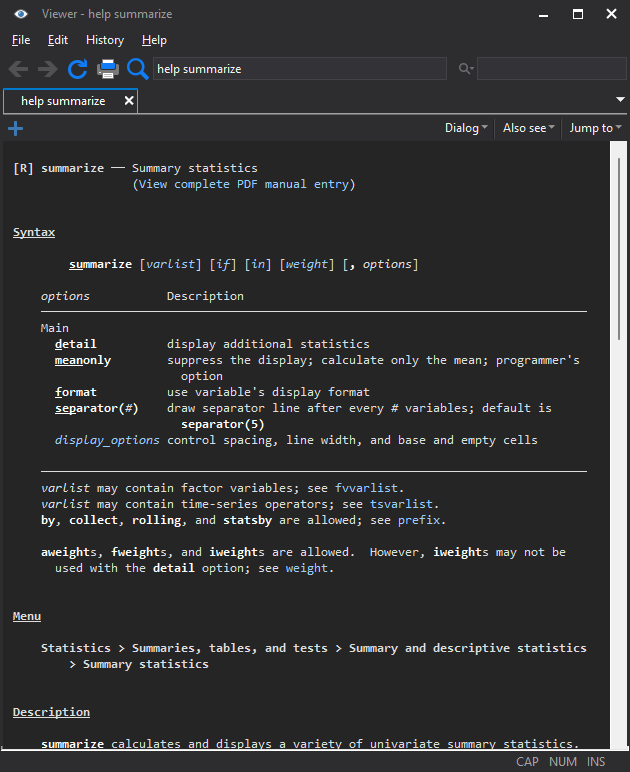
\includegraphics[width=0.85\textwidth]{helpsummarize}
\end{figure}

\subsection{Storing Information}

\subsubsection{Scalars and matrices}

Rather than storing information in variables,
Stata offers us a couple of different ways of storing information independently of a datset.
Scalars and matrices are perhaps the most basic of these options.
Other than the names suggest, scalars are not limited to containing only numbers:
we are free to store other types of information such as strings in them as well.
Matrices can only contain numerical values, on the other hand.
Another difference between the two is the amount of information stored:
a scalar contains a single piece of information,
whereas a matrix can contain multiple pieces of information.

Scalars can be created using the \st{scalar define} command,
although the \st{define} can be left out.
For example,
if I want to create a scalar containing the number 7,
I could type:
\begin{minted}{stata}
  scalar define number = 7
\end{minted}

After running this line of code -- either through a do-file or the Stata console -- Stata has now created a scalar with the name ``number'' that contains the numerical value 7.
Naturally, we cannot always remember every piece of information we have stored.
If we want to know what scalars currently exist in Stata's memory, we use another command:
\begin{minted}{stata}
  scalar define number = 7
  scalar define second = "two"
  scalar list
\end{minted}
After running the second command, Stata returns us a list of all scalars with both their name and value:
\small\begin{verbatim}
  . scalar list
      second = two
      number =          7
\end{verbatim}\normalsize
Note that we can also type \st{dir} instead of \st{list} and obtain the same result.

Compared to scalars, matrices are both more versatile and more complicated to work with.
As they store multiple pieces of information, every piece of information also needs a position.
Creating a matrix is slightly different compared to creating a scalar:
\begin{minted}{stata}
  matrix input numbers = ( 7 , 2 \ 1 , 2)
\end{minted}
This creates a two by two matrix (i.e.\ two rows and two columns),
containing the values 7 and 2 in the first row and the values 1 and 2 in the second row.
In this command, commas seperate row values while backslashes start a new row.
Again, \st{input} can be omitted when creating a matrix.
There is also a \st{matrix define} command,
but this is used when we do computations with already existing matrices.
\st{input} is used when inputting matrices by hand.

To see existing matrices, we use two commands:
\begin{minted}{stata}
  matrix input numbers = ( 7 , 2 \ 1 , 2)
  matrix dir
  matrix list numbers
\end{minted}
The first of these shows us a list of all matrices in Stata's memory and their size,
while the second command shows us the values of the matrix called ``numbers'':
\small\begin{verbatim}
  .   matrix dir
        numbers[2,2]

  .   matrix list numbers

  numbers[2,2]
      c1  c2
  r1   7   2
  r2   1   2
\end{verbatim}\normalsize

Finally,
we can remove scalars and matrices from Stata's memory using their respective command followed by \st{drop}:
\begin{minted}{stata}
scalar drop _all
matrix drop numbers
\end{minted}
We can remove a specific scalar or matrix by specifying its name,
or we can remove all existing scalars or matrices by typing \st{_all} instead of a name.
Scalars and matrices are also removed from memory when you close Stata itself or when you issue the \st{clear all} command.

The \st{help} file for both commands provide a lot more information on both scalars and matrices, especially so for the latter.
Also note that, especially for matrices, a lot is possible using Stata's underlying programming language Mata.
Unless you plan on writing elaborate and complex estimation commands,
you will likely never need or encounter Mata;
it is thus beyond the scope of this reader -- for now.\footnote{~At the moment, I do not have a lot experience with Mata yet, either. Although writing a guide on it would likely be a quick way for me to learn it, I do not it would add much value for the reader. I might change my mind about this later, though.}

\subsubsection{Macros}

Stata recognises two types of macros: \st{global}s and \st{local}s.
If you are not familiar with the term,
a macro is basically a shorthand or abbreviation:
instead of repeatedly typing out some very long string of characters,
we can define and use a macro instead, saving space, time,
and keeping our code much more organised.

\paragraph{Locals}
Of the two macro types, the local is most common.
The major (dis)advantage of a local is that Stata ``forgets'' it after running the code it is defined in.
This means we cannot use locals interactively:
if we define a local in Stata's command line,
it will be gone by the time we execute a second command.
At the same time,
this also means we can repeatedly redefine the contents of a local without having to drop it after every time we run a block of code,
and, more importantly, locals in our programs won't interfere with locals of other programs.

The basic syntax for defining a local is relatively simple:
\begin{minted}{stata}
local name contents
\end{minted}
All we need is to indicate that we are defining a \st{local}, give it a name,
and provide its content.
To use the local, we need to tell Stata to expand it in our following command(s).
We do this by surrounding the local's name by a single opening and closing quote, i.e. \st{`name'}.
Note that you \emph{have} to use the separate opening and closing quote characters,
using a single closing quote twice --
as you would in a regular text processor such as Word\footnote{%
~Most modern text processors automatically change the straight quotes of our keyboard into opening or closing quotes,
depending on the surrounding characters.
Most programming environments don't:
you generally aren't writing text in a programming environment, but code.} --
will generally cause Stata to return an error,
as it does not recognise our local as such.
In short: write \st{`name'}, not \st{'name'}.

To make the concept a little less abstract, I'll provide an example.
Suppose you have a large amount of regressions or other estimation commands you want to run,
all with the same control variables.
Instead of typing out all the variable names every time,
we can define a local with the variable names and use that instead.
\cref{lst:local} does just this, and you can copy the code\footnote{the code is also available to download as a do-file on the reader's GitHub page \href{https://github.com/Ahvns/ETPreader/tree/main/Example\%20do-files}{here}. Later example codes will all be available to download there as well.} into a do-file and try for yourself.

\begin{listing}[htp]
\caption{using a local for control variables}\label{lst:local}
\inputst{local.do}
\end{listing}
\subsection{display}

display command
